\section{相关背景}

本章节将介绍矢量数据库的相关背景,包括矢量数据的类型和矢量的相关算法,为后续矢量数据库及其原理讲解作前置铺垫。

\subsection{矢量的定义和表示}

矢量(或称向量),是由数值组成的数据集合,一个矢量表示一个多维空间中的点或特征。每个矢量由一组有序的数值组成,这些数值可以是实数或离散值。在矢量数据中,每个维度代表了矢量的一个特征或属性。例如,如果考虑一个二维矢量数据集,每个矢量可以表示平面上的一个点,其中第一个维度表示横坐标,第二个维度表示纵坐标。一个矢量可以有如下表示:

\begin{equation}
    V=\{v_1,v_2,\dots,v_n\}\in\mathbb{R}^{n},
    \label{eq:def_vector}
\end{equation}

如公式\ref{eq:def_vector}所示,$n$维矢量$V$中包含若干元素$v_1,v_2,\dots,v_n$,其中每个元素$v_i$都是一个数值,拥有其特定含义或属性。

在机器学习、深度学习等领域中,矢量数据拥有了更为高维的含义。机器学习通常通过人工标注的特征进行学习,例如可以将图像分解出颜色直方图、纹理特征、形状描述符等特征,之后将这些特征拼接组织成矢量后,就可以进行后续的分类、回归等任务。在深度学习中,矢量的含义则更加难以解释,由于深度学习依赖的特征数量极多,不可能逐一进行人工标注。因此深度学习模型得到的特征矢量往往是自学习的,每个特征拥有不同的含义,维度很多又难以解释。因此,矢量数据的组织和存储是很大的难题。

\subsection{矢量的类型}

从应用领域来看,矢量具有以下典型的类型:

\begin{itemize}
\item 图像特征矢量。在计算机视觉中,图像可以表示为一系列特征矢量。每个特征矢量可能代表图像中的某个区域或特定的视觉特征,这些特征可能是人工的,如颜色直方图、纹理特征或形状描述符,也可能是深度模型自学习的。
\item 文档矢量。在文本挖掘和自然语言处理中,文档可以表示为矢量。每个文档矢量可能表示文档中单词的出现频率、TF-IDF值或其他文本特征,当然也可能是自学习的。
\item 用户偏好矢量。在推荐系统中,可以使用用户的行为数据来构建用户偏好矢量。每个用户偏好矢量表示用户对不同项目或特征的偏好程度。
\item 传感器数据矢量。在物联网和传感器网络中,传感器收集的数据可以表示为矢量。每个矢量可能包含不同传感器的测量值,如温度、湿度、压力等。
\item 基因表达式矢量。在生物信息学中,基因表达数据可以表示为矢量。每个矢量表示基因在不同样本或实验条件下的表达水平。
\end{itemize}

目前,各种科研和工程领域都需要存储和分析大量矢量数据,因此矢量数据库对于各大领域来说都有很大的需求,前景广泛。

\subsection{矢量的相关算法}

在机器学习中,常见的算法可以分为分类、回归、聚类等任务,这些任务都需要依赖矢量才能进行。例如,分类和回归算法通常需要根据矢量中的特征,经过某种变换映射到标签上;而聚类算法通常需要通过度量矢量之间的关系,将矢量自适应的分为若干类簇。以经典算法K近邻分类\cite{keller1985fuzzy}为例,对于一个待分类的样本来说,需要计算距离该样本最近的K个样本,之后统计这K个样本中出现最多的类别,从而认为该样本属于该类别。

\begin{figure}
    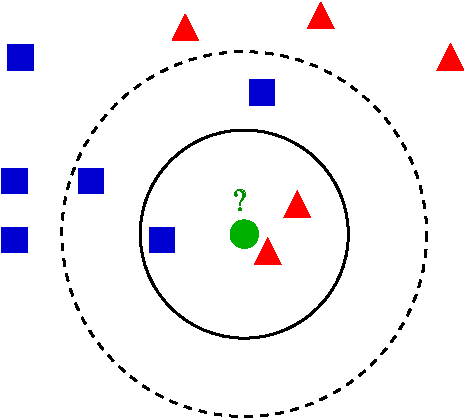
\includegraphics[width=0.5\textwidth]{examples/knn.pdf}
    \centering
    \caption{KNN分类算法示例}
    \label{fig:knn}
\end{figure}

图\ref{fig:knn}是一个典型的K近邻分类示例,图中不同的颜色/形状代表不同的类型,待分类对象是绿色圆点。当$K=3$时,最近的3个样本如实线圆圈所示,出现最多的样本为红色三角形,因此待分类对象也被认为是红色三角形。当$K=5$时情况发生了改变,出现最多的样本是蓝色正方形,因此待分类对象也被认为是蓝色正方形。算法的效果与参数K有很大的关系。

那么如何度量两个矢量之间的距离以找到最近的样本?一种常见方案是计算矢量的欧氏距离。

\begin{equation}
    D(V^1,V^2)=\sqrt{(v_1^1-v_1^2)^2+(v_2^1-v_2^2)^2+\dots+(v_n^1+v_n^2)^2},
    \label{eq:knn}
\end{equation}

公式\ref{eq:knn}展示了欧氏距离的计算方式,其中$V^1,V^2$代表两个矢量,$v_i^j$代表第$j$个矢量的第$i$个元素。通过对该案例的分析,可以发现机器学习需要对矢量和矢量之间进行大量分析和统计,其余领域也是如此。因此,对于矢量的分析能力也是矢量数据库的一大需求。